%%%%%%%%%%%%%%%%%%%%%%%%%%%%%%%%%%%%%%%%%%%%%%%%%%%%%%%%%%%%
%% Chapter 5 — Learned Models and Online Adaptation
%% Target length: 14 pages.
%% Purpose: develop the learned actuator representations, their
%% training objectives, and the adaptation chain; separate what the
%% evidence establishes and the scope of each result.
%% Deployment-level gate results belong to Chapter 7 and are not
%% repeated here.
%%%%%%%%%%%%%%%%%%%%%%%%%%%%%%%%%%%%%%%%%%%%%%%%%%%%%%%%%%%%
\chapter{Learned Models and Online Adaptation}
\label{chap:models}

Chapter~\ref{chap:data} established how the datasets were generated and why
both closed-loop operation and open-loop valve excitation were required. This
chapter develops the learned representations that consume them: the
inverse-dynamics (ID) and forward-dynamics (FD) networks of the \ppoIDFD{}
actuator path, the command-conditioned reduced-order model (ROM) that replaces
them in \ppoROM, and the system-dynamics surrogate, privileged factor encoder
and Arm Adaptation Module (AAM) that together carry the adaptation argument.

Two commitments organise the chapter. The first is that the surrogate is kept
strictly separate from the deployed actuator: the system-dynamics model is an
instrument for establishing whether a compact dynamics latent exists and is
useful, never a component of any control stack. The second is that no model is
accepted on a supervised score, because a recurring result of this work is that
such scores can be not merely optimistic but uninformative: a forward model
reached a one-step $R^2$ near $0.999$ while having learned almost nothing about
valve authority (Section~\ref{sec:models:fd}). Every model is therefore
presented with its contract, training objective, and the offline evidence that
accepted or refused it. All models operate on cylinder-space signals; the
mapping to task space belongs to Chapter~\ref{chap:system}, the control
integration to Chapter~\ref{chap:control}, and deployment-level results to
Chapter~\ref{chap:evaluation}.

\section{Modelling Overview and Common Notation}
\label{sec:models:overview}

All learned models act on the four hydraulic cylinders of the MULAG arm,
indexed $i \in \{1,\dots,4\}$ in the fixed order slew cylinder
(\emph{Drehzapfen}), boom cylinder~I (\emph{Ausleger~I}), boom cylinder~II
(\emph{Ausleger~II}) and head pivot cylinder (\emph{Messerkopf-Schwenk}). The
passive fifth joint is not actuated and enters no model input. At the
learned-model sample time $T = \unit[0.05]{s}$ the discrete index $k$ refers to
the cylinder extension $\bm{x}_k$, the extension velocity $\dot{\bm{x}}_k$, the
chamber pressure difference $\Delta\bm{p}_k$ and the logged rod force
$\bm{F}_k$, each in $\mathbb{R}^4$. The valve command
$\bm{u}_k \in [-1,1]^4$ is the normalised spool command of the four
proportional valves. The desired cylinder command produced by the task
controller is the pair
%
\begin{equation}
  \label{eq:models:command}
  \bm{c}_k = \bigl[\Delta\bm{x}^{*}_k,\; \Delta\dot{\bm{x}}^{*}_k\bigr]
  \in \mathbb{R}^{8},
\end{equation}
%
the extension and extension-velocity increments to be realised over the next
sample. Predictions carry a hat, and $\Delta(\cdot)_k = (\cdot)_{k+1} -
(\cdot)_k$ denotes a within-run one-step increment throughout.

\begin{figure}[tbp]
  \centering
  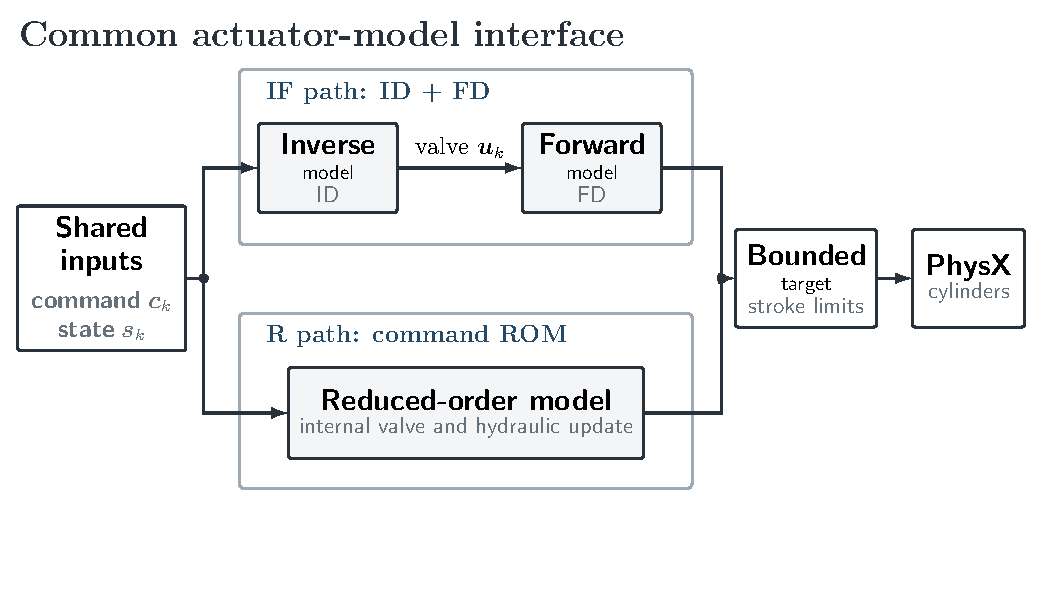
\includegraphics[width=\textwidth]{images/models_overview}
  \caption{Common interface of the two alternative actuator paths. Both
  receive the desired cylinder command and measured hydraulic state, and both
  produce the same bounded PhysX cylinder target. The \ppoIDFD{} path composes
  the inverse and forward models; the \ppoROM{} path uses one
  command-conditioned reduced-order model.}
  \label{fig:models:overview}
\end{figure}

Figure~\ref{fig:models:overview} compares the actuator paths. In \ppoIDFD, the
ID maps the state and desired increment to a valve command, and the FD predicts
the resulting increment. In \ppoROM, one command-conditioned model predicts
the valve internally and propagates pressure, velocity and extension. Both
paths produce the same bounded PhysX cylinder target in
IsaacLab~\cite{mittal2023orbit} under the same policy action
contract~\cite{schulman2017proximal}.

Three conventions apply throughout. Dynamic targets are within-run increments,
with $\Delta\hat{\bm{x}}=\bm{0}$ as the persistence baseline. Each checkpoint
uses its own training-set normalisation. Inputs at step $k$ are causal, and
targets are measured transitions to step $k+1$.

Simscape supplies the identification data described in Chapter~\ref{chap:data}.
The exported arrays are audited, frozen and used to train the models in
PyTorch~\cite{paszke2019pytorch}; Simscape is not part of training or
deployment.

The closed-loop Simscape export~\cite{mathworks2024simscape} contains
$452\,400$ transitions at $T=\unit[0.05]{s}$ from $1\,040$ runs, split by run
into $936/52/52$ training, validation and test runs. It supplies the supervised
ID, FD and command-ROM data. The FD repair uses four open-loop $64$-s runs at
$\unit[0.01]{s}$ with rank-4 valve excitation on four plant draws.

\section{Inverse Dynamics Model}
\label{sec:models:id}

The ID network maps the current hydraulic state and desired cylinder increment
to a valve-command change:
%
\begin{equation}
  \label{eq:models:id-contract}
  \Delta\bm{u}_k = f_{\mathrm{ID}}
  \bigl(\bm{x}_k,\, \dot{\bm{x}}_k,\, \Delta\bm{p}_k,\, \bm{F}_k,\,
        \Delta\bm{x}^{*}_k,\, \Delta\dot{\bm{x}}^{*}_k,\, \bm{u}_{k-1}\bigr)
  \in \mathbb{R}^4 ,
\end{equation}
%
a 28-dimensional input. The deployed command is
$\bm{u}_k = \operatorname{clip}(\bm{u}_{k-1} + \Delta\bm{u}_k,\,
-\bm{u}_{\max},\, \bm{u}_{\max})$ with per-axis limits
$\bm{u}_{\max} = [0.95,\, 0.95,\, 0.8,\, 0.8]$ stored in the checkpoint.
The change formulation retains the previous valve operating point near the
direction-dependent dead zone (Section~\ref{sec:fund:actuation-chain}). Logged
achieved transitions serve as desired increments because no independent
cylinder-space reference was recorded.

The 512-wide residual MLP~\cite{he2016deep} uses SiLU activations, layer
normalisation and dropout~\cite{elfwing2018sigmoid,ba2016layer,srivastava2014dropout}.
Adam minimises a smooth-$L_1$ loss on normalised targets, with saturated samples
up-weighted~\cite{kingma2015adam,huber1964robust}.

Figure~\ref{fig:models:id-architecture} separates the three input groups and
shows the four residual blocks explicitly. The network predicts a four-axis
valve-command increment, which is accumulated and clipped before use.

\begin{figure}[H]
  \centering
  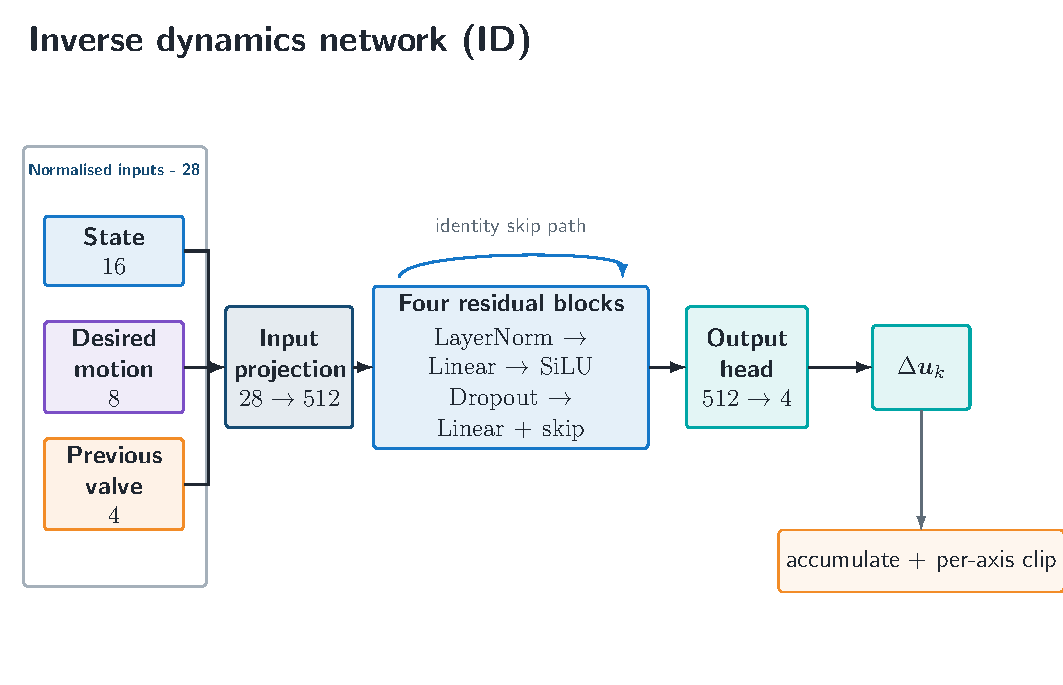
\includegraphics[page=1,width=\textwidth]{images/ch5_network_architectures}
  \caption{Inverse-model architecture. Current hydraulic state (16), desired
  motion (8) and the previous valve command (4) form the 28 inputs. A
  512-wide, four-block residual MLP predicts $\Delta\bm{u}_k$, which is
  accumulated and clipped per axis to form the bounded valve command.}
  \label{fig:models:id-architecture}
\end{figure}

Per-valve validation $R^2$ is $0.9973$--$0.9996$. This shows reproduction of
logged commands, not plant authority: in closed-loop data, achieved transitions
and logged commands are correlated (Section~\ref{sec:fund:identifiability}).

\subsection{Paired Control Fine-Tuning}
\label{sec:models:id-paired}

The composite is assessed by the \emph{paired differential response}: the FD
prediction under the ID command for the requested target minus the prediction
under its command for a zero target,
%
\begin{align}
  \bm{u}^{\mathrm{tgt}}_k &= f_{\mathrm{ID}}(\cdot,\, \bm{c}_k,\, \bm{u}_{k-1}),
  \qquad
  \bm{u}^{0}_k = f_{\mathrm{ID}}(\cdot,\, \bm{0},\, \bm{u}_{k-1}), \notag \\
  \Delta\hat{\bm{x}}^{\mathrm{pair}}_k &=
    f_{\mathrm{FD}}\bigl(\bm{u}^{\mathrm{tgt}}_k, \cdot\bigr)
  - f_{\mathrm{FD}}\bigl(\bm{u}^{0}_k, \cdot\bigr).
  \label{eq:models:paired}
\end{align}
%
Before fine-tuning, the composite normalised control error was $1.00$, equal to
the zero-response baseline, and all regression slopes were below $0.004$
(Table~\ref{tab:models:paired}). The networks were fine-tuned jointly on
$\mathcal{L}_{\mathrm{ctl}} = \| \Delta\hat{\bm{x}}^{\mathrm{pair}}
- \Delta\bm{x}^{*} \|^2_{\mathrm{norm}}
+ \lambda_{\mathrm{ID}}\mathcal{L}_{\mathrm{ID}}
+ \lambda_{\mathrm{FD}}\mathcal{L}_{\mathrm{FD}}$,
with the supervised terms retained. Target blocks were shuffled across valid
states to break the logged state--target pairing. After 30 epochs, control
error fell to $0.109$; all slopes exceeded $0.8$ and all correlations exceeded
$0.92$. This frozen checkpoint is used in \ppoIDFD{} and \ppoAAMIDFD{}.

\begin{table}[H]
  \centering
  \caption{Effect of paired control fine-tuning on the composite differential
  response \eqref{eq:models:paired}, per cylinder axis on validation data.
  Before fine-tuning the composite had essentially no control authority despite
  near-perfect supervised scores of both networks; the composite normalised
  control error fell from $1.0011$ to $0.1086$.}
  \label{tab:models:paired}
  \begin{tabular}{lcccc}
    \toprule
    & \multicolumn{2}{c}{Regression slope}
    & \multicolumn{2}{c}{Correlation} \\
    \cmidrule(lr){2-3} \cmidrule(lr){4-5}
    Cylinder axis & before & after & before & after \\
    \midrule
    1 (slew)      & $0.003$ & $0.818$ & $0.135$ & $0.920$ \\
    2 (boom I)    & $0.002$ & $0.928$ & $0.090$ & $0.967$ \\
    3 (boom II)   & $0.001$ & $0.849$ & $0.037$ & $0.933$ \\
    4 (head pivot)& $0.004$ & $0.912$ & $0.249$ & $0.958$ \\
    \bottomrule
  \end{tabular}
\end{table}

\subsection{Transfer of the Frozen Inverse Model}
\label{sec:models:id-trust}

Because the adapter corrects a frozen ID, its transfer was checked on a separate
$64$-run IsaacLab collection: $2$ nominal, $16$ hydraulic-only, $12$
mechanical-only and $34$ combined runs. These runs do not overlap the $118$-run
adaptation collection. They are also outside the ID training distribution,
which contains only Simscape data. Evaluation was teacher-forced at each ROM
tick and scored on the predicted valve command.

The recorded valve RMS is $0.4350$ and the ID error is $0.1739$, corresponding
to about $84\,\%$ explained command variance. Domain-mean error varies by only
a factor of $1.09$ (Table~\ref{tab:models:id-trust}); the nominal domain is not
the easiest.

\begin{table}[tb]
  \centering
  \caption{Transfer of the frozen inverse model across deployment domains,
  $64$ runs, teacher-forced at the ROM tick. The error is on the valve command,
  the model's own output. The recorded valve signal has RMS magnitude $0.4350$.
  The spread across domains is a factor of $1.09$; nominal is not the easiest
  domain.}
  \label{tab:models:id-trust}
  \begin{tabular}{lcccc}
    \toprule
    Domain & runs & valve RMSE & s.d. & worst run \\
    \midrule
    combined   & $34$ & $0.1739$ & $0.0311$ & $0.2917$ \\
    hydraulic  & $16$ & $0.1672$ & $0.0170$ & $0.2174$ \\
    mechanical & $12$ & $0.1828$ & $0.0129$ & $0.2082$ \\
    nominal    & $2$  & $0.1829$ & $0.0155$ & $0.1984$ \\
    \bottomrule
  \end{tabular}
\end{table}

Three limitations remain. As a one-step state predictor, the ID gives
$\unit[1.002]{mm}$ extension error versus $\unit[1.143]{mm}$ for zero-order
hold, while zero-order hold is $8\,\%$ better on velocity. Recursive composite
rollout diverges in $48$ of $64$ runs; mean valve-saturation occupancy is
$0.989$ in diverging runs and $0.223$ in stable runs. This does not affect the
one-step closed-loop use. Finally, measured pressure input increases extension
error from $\unit[1.311]{mm}$ to $\unit[1.907]{mm}$, so deployment uses the
training-mean pressure.

\section{Forward Dynamics Model}
\label{sec:models:fd}

The FD network predicts the one-step cylinder response to a valve command,
%
\begin{equation}
  \label{eq:models:fd-contract}
  \bigl[\Delta\hat{\bm{x}}_k,\; \Delta\hat{\dot{\bm{x}}}_k,\;
        \Delta\widehat{\Delta\bm{p}}_k\bigr]
  = f_{\mathrm{FD}}\bigl(\bm{u}_k,\, \bm{x}_k,\, \dot{\bm{x}}_k,\,
    \Delta\bm{p}_k,\, \bm{F}_k\bigr) \in \mathbb{R}^{12},
\end{equation}
%
using the same residual trunk as the ID network. Supervised pretraining on the
closed-loop export, with an auxiliary recursive rollout
loss~\cite{nagabandi2018neural}, reached grouped one-step $R^2$ near $0.999$
for the extension increments.

Figure~\ref{fig:models:fd-architecture} shows the forward model separately
because its input and output contracts differ from the inverse model despite
the shared residual trunk.

\begin{figure}[H]
  \centering
  \includegraphics[page=2,width=\textwidth]{images/ch5_network_architectures}
  \caption{Forward-model architecture. The applied valve command and cylinder
  state condition a one-step hydraulic transition through a 512-wide,
  four-block residual MLP. Its 12 outputs are extension, velocity and pressure
  increments. Extension is the integrated controller output; velocity and
  pressure are diagnostic outputs.}
  \label{fig:models:fd-architecture}
\end{figure}

\subsection{Assessment of the Supervised Score}
\label{sec:models:fd-identifiability}

The supervised score did not establish valve sensitivity. At a
$\unit[0.5]{s}$ horizon, zeroing the valve input changed the rollout-error
ratio to only $0.94$. The FD had mainly extrapolated the smooth closed-loop
kinematics because command and state history were nearly redundant. Closed-loop
ablation confirmed that the valve was not identifiable, so repair required new
data.

The repair dataset applies rank-4 open-loop valve plateaus to four plant draws.
Its trajectories are distinct, valve history predicts pressure with
$R^2\approx0.80$--$0.85$, valve-regressor variance-inflation factors are
$7$--$10$, and relief saturation occupies $9$--$22\,\%$ of samples. A previous
export with duplicated trajectories was rejected~\cite{isermann2011identification}.

Starting from the paired-control checkpoint, strict retraining minimised
%
\begin{equation}
  \label{eq:models:fd-strict-loss}
  \mathcal{L}_{\mathrm{FD}} =
    \mathcal{L}_{\mathrm{Huber}}^{\mathrm{strict}}
    + 0.25\, \mathcal{L}_{\mathrm{Huber}}^{\mathrm{MAT}}
    + 2.0\, \mathcal{L}_{\mathrm{roll}}^{(10)}
    + 10.0\, \mathcal{L}_{\mathrm{kin}},
\end{equation}
%
combining the one-step loss on the strict data, a replay term on the original
closed-loop data, a $\unit[0.5]{s}$ recursive rollout loss, and a kinematic
consistency term enforcing the trapezoidal identity
%
\begin{equation}
  \label{eq:models:trapezoid}
  \Delta\bm{x}_k = T\,\dot{\bm{x}}_k
  + \tfrac{1}{2}\, T\, \Delta\dot{\bm{x}}_k ,
\end{equation}
%
which holds in the strict data with $R^2=0.994$--$0.9997$. A constant valve
Jacobian was rejected because measured authority varies by a factor of
$15$--$75$ across pressure quartiles and can change sign. This operating-point
dependence motivates the ROM structure~\cite{merritt1967hydraulic}.

Strict retraining reduces extension rollout RMSE from $\unit[75.2]{mm}$ to
$\unit[12.4]{mm}$ at $\unit[0.5]{s}$ and from $\unit[157.9]{mm}$ to
$\unit[27.3]{mm}$ at $\unit[1.0]{s}$. The valve-zero error ratio rises from
$0.94$ to $1.81$, and per-axis one-step extension $R^2$ improves from
$[-5.7,\,0.60]$ to $[0.76,\,0.98]$. Zero-order hold remains competitive below
$\unit[0.25]{s}$, and velocity increments remain weak on two axes. Deployment
therefore integrates only $\Delta\hat{\bm{x}}$ and retains velocity as a
diagnostic output.

\section{Reduced-Order Model}
\label{sec:models:rom}

The \ppoROM{} path uses one command-conditioned model instead of the ID--FD
composition. Its structure is grey-box: physical equations propagate pressure,
force, velocity and extension. Neural heads estimate valve realisation, load
and bounded residuals~\cite{karniadakis2021physics,lutter2019deep}. Valve authority is
pressure dependent by construction through the orifice-flow and continuity
equations~\cite{merritt1967hydraulic}. A GRU~\cite{cho2014learning} reads six
samples ($\unit[0.25]{s}$) of cylinder state, previous predicted valve command
and desired command. The measured valve is only an internal-head training
target~\cite{hwangbo2019learning}.

\begin{figure}[H]
  \centering
  \includegraphics[page=3,width=\textwidth]{images/ch5_network_architectures}
  \caption{Command-conditioned ROM. A recurrent neural proposal encodes a
  six-step history. Its actuation, bounded-residual and load heads condition
  the explicit hydraulic update: orifice flow, pressure, force, velocity and
  position. The explicit chain constrains the predicted transition.}
  \label{fig:models:rom-structure}
\end{figure}

The actuation head uses a learnable smooth dead zone with per-cylinder width
and asymmetric gains~\cite{yang2026stateconstrained}. Its output
$\hat{a}_i\in[-1,1]$ drives the orifice-flow and continuity update
%
\begin{align}
  q_i &= \hat{a}_i\, k_{q,i}\,
    \sqrt{\tfrac{1}{2}\bigl(p_{s,i} - \operatorname{sgn}(\hat{a}_i)\,
    \Delta p_i\bigr)_{+}}, \notag \\
  \Delta \hat{p}_{i,k+1} - \Delta p_{i,k} &=
    \frac{4\beta_i}{V_i(x_i)}
    \bigl(q_i - A_i \dot{x}_i - k_{\ell,i}\, \Delta p_i\bigr)\, T
    \;+\; r_{p,i},
  \label{eq:models:rom-pressure}
\end{align}
%
where $\beta_i$, $p_{s,i}$, $k_{q,i}$, $k_{\ell,i}$, $A_i$ and $V_i(x_i)$ are
the effective bulk modulus, supply pressure, flow gain, leakage, piston area
and chamber volume. Pressure then produces force and motion:
%
\begin{align}
  \hat{F}_i &= \Delta\hat{p}_{i,k+1} A_i + r_{F,i}, \qquad
  \ddot{x}_i = \frac{\hat{F}_i - c_{v,i}\,\dot{x}_i - \ell_i(\bm{h}_k)}{m_i},
  \notag \\
  \dot{\hat{x}}_{i,k+1} &= \dot{x}_{i,k}
    + \operatorname{sat}\bigl(T\,\ddot{x}_i + r_{v,i}\bigr), \qquad
  \hat{x}_{i,k+1} = x_{i,k}
    + \tfrac{T}{2}\bigl(\dot{x}_{i,k} + \dot{\hat{x}}_{i,k+1}\bigr)
    + r_{x,i},
  \label{eq:models:rom-motion}
\end{align}
%
Here $c_{v,i}$ is viscous friction, $m_i$ is effective modal mass and
$\ell_i(\bm{h}_k)$ is the learned configuration-dependent load. Physical
parameters are trained in log-space inside fixed clamps. Several settle on a
clamp bound and are therefore fitting coefficients rather than measured
constants: modal mass and viscous friction both reach their upper clamp of
$10^{7}$ (in kilograms and in newton-seconds per metre respectively), the
piston area reaches its lower clamp of $\unit[1]{cm^2}$ against a
$\unit[64]{cm^2}$ initialisation, and the supply pressure separates onto both
clamps, with two cylinders at $\unit[1]{MPa}$ and two at $\unit[50]{MPa}$. The
same values appear in every checkpoint of this family. Pressure and velocity
residuals are bounded to $10\,\%$ of their step limits, and the position
residual to $\unit[1]{cm}$, capping the magnitude each head may add per step.

The explicit chain and the neural heads contribute to the transition in very
different proportions. With the residual heads inactive the explicit chain
alone produces no net travel, its velocity increments falling six orders of
magnitude below their nominal values: at the fitted parameters the friction
term $c_{v,i}\dot{x}_i$ reaches $\unit[1.0]{MN}$ at $\unit[0.1]{m/s}$, against
a pressure force $\Delta\hat{p}_{i}A_i$ of about $\unit[10]{kN}$ at
$\unit[100]{MPa}$. Realised displacement is produced by the residual heads.
The pressure equation nonetheless remains active and responsive to its own
parameters: with the heads inactive, halving $k_{\ell,i}$ still moves
$\Delta p$ by $63\,\%$ of its range. Hydraulic parameters therefore reach the
predicted motion indirectly, through the pressure state entering the recurrent
encoder, rather than through the force balance. The model is grey-box in
structure---the equations fix the functional form of the transition and keep it
differentiable in named hydraulic quantities---rather than an identification of
the machine's physical constants.

Training uses rollout horizons $H\in\{1,5,20,50\}$ and scheduled sampling up to
$75\,\%$ self-fed~\cite{bengio2015scheduled}. Residual penalties retain the
physical structure. Logged rod force has zero supervised weight because PhysX
generates it at deployment and the export fails the piston-area consistency
check.

With the true command, mean one-step $R^2$ is $0.998$ for the internal valve,
$0.64$ for velocity and $0.97$ for extension. Zeroing or shuffling the command
reduces velocity $R^2$ below zero and extension to about $0.5$; the extension
Jacobian is diagonally dominant with condition number $2.14$. At
$\unit[5]{s}$, terminal extension $R^2$ is $0.998$, $0.998$, $0.84$ and $0.91$
across the cylinders. Pressure-increment $R^2$ is only $0.06$--$0.09$, so the
internal pressure is a dynamic state, not a calibrated pressure estimate
(Figure~\ref{fig:models:rom-validation}).

\begin{figure}[H]
  \centering
  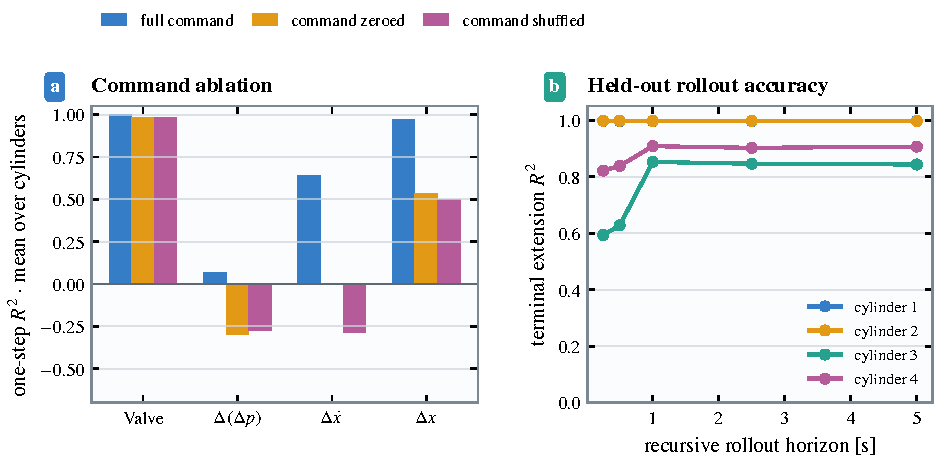
\includegraphics[width=\textwidth]{images/ch5_rom_validation}
  \caption{Offline validation of the command ROM on held-out runs.
  (a)~One-step $R^2$ per output group, averaged over the four cylinders, with
  the full desired command, with the command zeroed, and with the command
  shuffled across the batch. The collapse of the velocity and extension scores
  without the true command demonstrates command authority. (b)~Terminal
  extension $R^2$ of recursive rollouts up to $\unit[5]{s}$, shown separately
  for each cylinder so coincident high-accuracy traces remain visible.}
  \label{fig:models:rom-validation}
\end{figure}

\subsection{Closed-Loop Calibration Against the Deployment Plant}
\label{sec:models:rom-calibration}

The Simscape-trained ROM has a systematic extension offset when driving PhysX.
The promoted checkpoint adds a bounded, command-gated correction:
%
\begin{equation}
  \label{eq:models:rom-correction}
  \hat{x}_{i,k+1} \leftarrow \hat{x}_{i,k+1} + \delta_i(\bm{h}_k, \bm{c}_k),
  \qquad |\delta_i| \leq \unit[3]{mm},
  \qquad \delta_i\big|_{\bm{c}_k = \bm{0}} = 0,
\end{equation}
%
It is trained on $4\,084$ IsaacLab transitions from five reachable reference
shapes, with Simscape replay. All hydraulic and integration parameters remain
frozen. The gate sets the correction to zero for a commanded hold.

The calibrated command ROM serves as the deployment plant in
Section~\ref{sec:sys:rom-is-plant}. Unlike the ID--FD path, it has seen PhysX
data. It is frozen and has no latent input; adaptation modifies only the inverse
path.

\section{The Privileged Latent and Its Limits}
\label{sec:models:latent}

The system-dynamics model is an analysis model, not an actuator. It approximates
the command-ROM--PhysX plant and tests whether a compact factor-dependent
context improves prediction. It is trained from scratch on the IsaacLab data
of Section~\ref{sec:data:isaaclab}.

At each $\unit[50]{ms}$ step, the model predicts the next 12-dimensional
hydraulic-state increment from the observable state, joint context, consecutive
commands $[\bm{u}_{k-1},\bm{u}_k]$ and a six-tick causal belief. Training uses a
five-transition unroll. The matched control $SD_0$ has the same structure but
no latent input.

The privileged encoder $\bm{z}=\mu(\bm{e})$ maps the six physical factors to two
dimensions and is trained jointly with $SD_z$. At a 20-tick horizon, the true
latent is compared with zero, shuffled, random, mean and nominal controls using
paired bootstrap intervals on validation and reserved-test runs.

The true latent reduces pooled rollout error by $7.20\times10^{5}$ on 20
validation runs ($95\,\%$ interval
$[-1.03\times10^{6},-4.30\times10^{5}]$) and by $4.41\times10^{5}$ on 16 test
runs ($[-7.61\times10^{5},-1.74\times10^{5}]$).

The per-channel result is narrower (Table~\ref{tab:models:latent-channels}).
The significant gain is confined to pressure; extension and velocity intervals
cross zero on both pools. These are the channels used by the controller.

Figure~\ref{fig:models:sd-architecture} shows the two conditioning paths and
the transition model. The privileged factor encoder is used during training;
the belief GRU uses only causal state-action history.

\begin{figure}[H]
  \centering
  \includegraphics[page=4,width=\textwidth]{images/ch5_network_architectures}
  \caption{System-dynamics surrogate. The transition model combines a
  two-dimensional static plant context and a 16-dimensional causal dynamic
  belief with the hydraulic state, consecutive valve commands and joint
  context. A three-layer, 256-wide MLP predicts the transition; training uses
  a five-step unroll.}
  \label{fig:models:sd-architecture}
\end{figure}

\begin{table}[H]
  \centering
  \caption{Per-channel decomposition of the paired latent advantage at a
  $20$-tick horizon, pooled over $36$ runs. Values are the mean paired
  difference between the latent-conditioned model and the no-latent control,
  with a $95\,\%$ bootstrap interval; a negative value favours the latent for
  the pooled state error, and a positive value favours it for the per-channel
  errors as signed here. The advantage is confined to the pressure channel.}
  \label{tab:models:latent-channels}
  \begin{tabular}{lccc}
    \toprule
    Channel & mean paired difference & $95\,\%$ interval & excludes zero \\
    \midrule
    extension & $5.2\times10^{-5}$ & $[-3.6\times10^{-5},\; 1.4\times10^{-4}]$ & no \\
    velocity  & $-2.4\times10^{-4}$ & $[-7.1\times10^{-4},\; 2.4\times10^{-4}]$ & no \\
    pressure  & $1.75\times10^{5}$ & $[2.1\times10^{4},\; 3.3\times10^{5}]$ & yes \\
    \bottomrule
  \end{tabular}
\end{table}

Thus the two-dimensional context contains held-out hydraulic information, but
this test does not establish AAM accuracy or control improvement. It compares
separately trained models; the within-model latent substitution in
Section~\ref{sec:eval:predictive-utility} isolates latent input and also finds
extension and velocity sensitivity. The main limitation is that the strongest
signal lies in pressure, which the controller does not integrate.

The encoder, $SD_z$, belief module, normalisers, input mask, split and rollout
protocol are then frozen for downstream use.

\section{Arm Adaptation Module}
\label{sec:models:aam}

The AAM estimates $\hat{\bm{z}}=\mathrm{AAM}(\bm{H}_t)$ from deployment
history. Each row contains five joint positions, five joint velocities, four
cylinder pressure differences and four previous valve commands. A four-layer,
width-64 causal convolution processes 20 rows ($\unit[1.0]{s}$, 360 values).

The pressure values are recursive actuator-model states, not measurements:
they come from the command ROM in \ppoROM{} and the frozen FD in
\ppoAAMIDFD{}. The factor vector, true latent, reference, future rows and hidden
state are excluded. Using the previous valve command keeps each row causal.
Validation selected the shortest competitive history from $5$, $10$, $20$ and
$40$ ticks. Latent RMSE is $0.802$ on validation and $0.734$ on reserved test.

Inference runs at $\unit[20]{Hz}$ inside the $\unit[60]{Hz}$ control loop. The
adapter is bypassed until 20 rows are available. A causal five-prediction rolling
mean adds $\unit[250]{ms}$ lag. Reported results use this online smoother, not
the earlier non-causal full-run average.

\subsection{Information Content of the Estimated Latent}
\label{sec:models:aam-content}

Linear decoding from the per-run mean estimate gives $R^2=0.956$ for seal
condition, $0.448$ for compliance, $0.114$ for flow, $0.081$ for supply
pressure, $0.056$ for centre-of-mass offset and $-0.008$ for mass. The latent
therefore represents mainly seal condition. It is stable within a run but does
not refine over time.

Low-dimensional adapters can lose information when factors act through
different channels~\cite{liu2025frma}. This differs from the rapid-motor-
adaptation assumption that only task-relevant factor directions need to be
retained~\cite{kumar2021rma}: here the dominant seal-condition direction acts
through pressure, which the controller does not integrate. Estimating named
physical quantities would improve interpretation but requires an explicit
plant model~\cite{hu2026bayesian}.

\section{Latent-Conditioned Inverse-Model Adapter}
\label{sec:models:adapter}

The frozen ID produces $\bm{u}_{\mathrm{base}}=\mathrm{ID}(\bm{s},\bm{r})$.
The adapter adds a bounded latent-conditioned residual:
%
\begin{equation}
  \label{eq:models:adapter}
  \bm{u} = \operatorname{clip}\bigl(
    \bm{u}_{\mathrm{base}} + g_\psi(\bm{s}, \bm{r}, \bm{u}_{\mathrm{base}},
    \hat{\bm{z}})\bigr).
\end{equation}
%
Training minimises valve-command MSE at the exact ROM tick, with the residual
bounded to $0.15$. The ID, FD and policy are frozen during adapter training.
The \ppoAAMIDFD{} policy is separately latent-conditioned, so disabling the
residual restores the baseline actuator path but not the baseline actor. This
provides the single-variable adapter ablation used in
Chapter~\ref{chap:evaluation}.

Figure~\ref{fig:models:aam-architecture} shows the causal convolutional stack
and the bounded adapter that consumes its estimate. The upper part is the AAM;
the lower part shows where adaptation enters the frozen inverse-model path.

\begin{figure}[H]
  \centering
  \includegraphics[page=5,width=\textwidth]{images/ch5_network_architectures}
  \caption{AAM and bounded ID adapter. Four causal convolutional blocks map a
  20-step history of 18 observable features to the compact latent
  $\hat{\bm{z}}\in\mathbb{R}^2$. The adapter combines this estimate with the ID
  inputs and adds a limited, bounded correction to the frozen valve command.}
  \label{fig:models:aam-architecture}
\end{figure}

\subsection{Open-Loop Evidence}

The residual cap is $0.15$, and the frozen ID already explains about $84\,\%$
of valve-command variance (Section~\ref{sec:models:id-trust}). The adapter can
therefore make only small corrections. Section~\ref{sec:eval:predictive-utility}
tests latent information without this ceiling.

Three matched adapter arms use a zeroed, estimated or privileged latent. Across
five seeds, both latent arms improve validation loss over the zeroed arm in
$5/5$ cases. Mean paired improvements are $0.0037$ for the privileged latent
and $0.0118$ for the AAM estimate. The effect is consistent but small.

Masking pressure and force does not strengthen the result: the privileged
latent helps in only $2/5$ seeds and variance increases by about one order of
magnitude. The earlier single-seed improvement is not reproducible.

\subsection{Closed-Loop Evidence and Its Bound}
\label{sec:models:adapter-null}

Closed-loop ablations compare the full stack with zeroed, shuffled, frozen and
mean latents, plus a sham plant change. None consistently improves lateral
error, cut-height error or impacts.

Valve saturation limits the test: cylinder 1 is saturated for about $92\,\%$ of
the scored window, cylinder 2 for $67$--$82\,\%$, and cylinder 4 for
$50$--$57\,\%$. Control-effort ratios before and after the plant change are
$1.005$--$1.009$. A bounded additive correction has little authority under
these conditions~\cite{sofrony2024antiwindup}.

Reducing the lead cap lowers cylinder-1 saturation from $0.91$ to $0.14$ but
triples cut-height error. The task is therefore close to the plant capability
limit (Section~\ref{sec:sys:capability}).

\subsection{Propagation of the Latent Advantage}
\label{sec:models:chain}

The chain gate compares
$SD_0(\bm{s},\bm{u})$, $SD_z(\bm{s},\bm{u},\bm{z})$ and
$SD_z(\bm{s},\bm{u},\hat{\bm{z}})$ under the frozen protocol with paired
bootstrap intervals. Neither the true nor estimated latent improves extension
or velocity over $SD_0$ with an interval excluding zero. The estimate is not
worse than the true latent, so estimation is not the limiting stage. The
measurable advantage remains in pressure (Table~\ref{tab:models:latent-channels}).

Section~\ref{sec:eval:predictive-utility} finds the estimate comparable with the
privileged latent within one model, confirming that the AAM is not the main
loss. The missing link is a path from pressure information to the integrated
extension command with sufficient actuator headroom. Chapters~\ref{chap:evaluation}
and~\ref{chap:conclusion} examine this limit.

\section{Training and Model-Selection Protocol}
\label{sec:models:training}

Adaptation data are split $82/20/16$ into training, validation and reserved
test by complete run and factor configuration; windows do not cross run
boundaries. The 16 test runs are not used for model or hyperparameter selection.
$SD_z$ and $SD_0$ are selected on validation rollout, the AAM on downstream
rollout, and the adapter on validation command error. Table~\ref{tab:models:frozen}
records the selected checkpoints.

\begin{table}[H]
  \centering
  \caption{Provenance of each model in the adaptation chain. Frozen components
  are loaded unchanged and never receive gradients in this chapter.}
  \label{tab:models:frozen}
  \small
  \begin{tabular}{lll}
    \toprule
    Model & Status & Selected checkpoint \\
    \midrule
    Control ID            & frozen  & paired-control, Section~\ref{sec:models:id} \\
    Strict FD             & frozen  & strict-excitation, Section~\ref{sec:models:fd} \\
    Command ROM           & frozen  & PhysX-calibrated, Section~\ref{sec:models:rom-calibration} \\
    $SD_0$ (no latent)    & scratch & epoch $58$ \\
    $SD_z$ + encoder      & scratch & epoch $48$, frozen after the gate \\
    AAM                   & scratch & epoch $73$, $\unit[1.0]{s}$ causal CNN \\
    Latent adapter        & scratch & epoch $116$ \\
    \bottomrule
  \end{tabular}
\end{table}

The deployed adapter is trained and selected on recorded valve-command error.
This avoids the objective mismatch of an earlier next-state-loss variant. Each
component is evaluated on its stated training contract.
